\begin{comment}
\begin{tikzpicture}
\begin{axis}[height=0.2\textheight, width=0.35\textwidth, style={font=\scriptsize},grid=major,grid style={dotted},align=center,xlabel={Mode},ylabel={Order},zlabel={Speedup},title={Tlib-SB-P2}, xtick={1,2,3,4,5,6,7}, xticklabels={1,2,3,4,5,6,7}, ytick={2,3,4,5,6,7}, yticklabels={2,3,4,5,6,7}, point meta max=12, point meta min=1, zmin=1, zmax=15, ztick={1,5,10,15},zticklabels={1,5,10,15}, view={-15}{25}, xlabel style={yshift=2mm}, ylabel style={yshift=5mm}, zlabel style={yshift=-1mm,xshift=-4mm}]
\addplot3[surf, colormap = {whiteblack}{color(0cm)=(white);color(0.4cm) = (darkgray)}] %  colormap/blackwhite
coordinates{
(1.000,2.000,0.999) (1.000,3.000,1.001) (1.000,4.000,0.999) (1.000,5.000,0.998) (1.000,6.000,0.997) (1.000,7.000,1.008) 

(2.000,2.000,0.997) (2.000,3.000,0.964) (2.000,4.000,1.197) (2.000,5.000,1.898) (2.000,6.000,2.423) (2.000,7.000,2.473) 

(3.000,2.000,0.978) (3.000,3.000,1.005) (3.000,4.000,1.900) (3.000,5.000,3.598) (3.000,6.000,5.642) (3.000,7.000,11.260) 

(4.000,2.000,0.999) (4.000,3.000,1.002) (4.000,4.000,1.002) (4.000,5.000,3.282) (4.000,6.000,6.075) (4.000,7.000,9.580) 

(6.000,2.000,1.002) (6.000,3.000,0.999) (6.000,4.000,0.999) (6.000,5.000,0.999) (6.000,6.000,1.000) (6.000,7.000,10.218) 

(7.000,2.000,1.003) (7.000,3.000,0.987) (7.000,4.000,1.002) (7.000,5.000,1.001) (7.000,6.000,1.007) (7.000,7.000,1.004) 

};
\end{axis}
\end{tikzpicture}
\end{comment}
\begin{comment}
\begin{tikzpicture}
\begin{axis}[height=0.40\textheight,width=0.40\textwidth,style={font=\footnotesize},grid=major,grid style={dotted},align=center,xlabel={Kontraktionsmodus},ylabel={Tensorstufe},title={TLib-SB-P3},scaled ticks=false,zticklabel=\pgfmathprintnumber{\tick},zlabel={Verhältnis},view={-45}{45}, zlabel={Standardfehler [\%]}]
\addplot3[surf]
coordinates{(1.000,2.000,0.395) (1.000,3.000,1.035) (1.000,4.000,1.183) (1.000,5.000,0.461) (1.000,6.000,0.675) (1.000,7.000,0.968) 

(2.000,2.000,1.092) (2.000,3.000,2.408) (2.000,4.000,21.326) (2.000,5.000,27.379) (2.000,6.000,28.588) (2.000,7.000,20.609) 

(3.000,2.000,4.428) (3.000,3.000,2.964) (3.000,4.000,35.937) (3.000,5.000,30.533) (3.000,6.000,28.414) (3.000,7.000,8.862) 

(4.000,2.000,1.226) (4.000,3.000,0.704) (4.000,4.000,0.531) (4.000,5.000,27.877) (4.000,6.000,22.175) (4.000,7.000,23.399) 

(6.000,2.000,0.400) (6.000,3.000,0.388) (6.000,4.000,0.308) (6.000,5.000,0.172) (6.000,6.000,0.379) (6.000,7.000,13.745) 

(7.000,2.000,0.356) (7.000,3.000,3.509) (7.000,4.000,0.523) (7.000,5.000,0.198) (7.000,6.000,1.904) (7.000,7.000,0.545) 

};
\end{axis}
\end{tikzpicture}
\end{comment}
\begin{tikzpicture}
\begin{axis}[height=0.2\textheight, width=0.35\textwidth, style={font=\scriptsize},grid=major,grid style={dotted},align=center,xlabel={Mode},ylabel={Order},zlabel={Speedup},title={\ttt{TLIB-LB-PN:TCL}}, xtick={1,3,5,7}, xticklabels={1,3,5,7}, ytick={3,5,7}, yticklabels={3,5,7}, point meta max=17, point meta min=1, zmin=1, zmax=17, ztick={1,9,17},zticklabels={1,9,17}, view={-35}{45}, xlabel style={yshift=2mm}, ylabel style={yshift=5mm}, zlabel style={yshift=-1mm,xshift=-4mm},title style={yshift=-2mm}] % zmode=log, 
\addplot3[surf] % , colormap = {whiteblack}{color(0cm)=(white);color(0.4cm) = (darkgray)}
coordinates{
(1.000,2.000,2.052) (1.000,3.000,1.689) (1.000,4.000,1.710) (1.000,5.000,1.402) (1.000,6.000,1.316) (1.000,7.000,1.319) 

(2.000,2.000,16.300) (2.000,3.000,2.646) (2.000,4.000,1.882) (2.000,5.000,1.582) (2.000,6.000,0.917) (2.000,7.000,0.460) 

(3.000,2.000,16.172) (3.000,3.000,7.333) (3.000,4.000,2.657) (3.000,5.000,2.382) (3.000,6.000,1.952) (3.000,7.000,2.287) 

(4.000,2.000,16.325) (4.000,3.000,7.330) (4.000,4.000,3.842) (4.000,5.000,2.513) (4.000,6.000,2.746) (4.000,7.000,2.561) 

(6.000,2.000,16.050) (6.000,3.000,7.333) (6.000,4.000,4.051) (6.000,5.000,3.228) (6.000,6.000,2.671) (6.000,7.000,2.709) 

(7.000,2.000,16.598) (7.000,3.000,7.285) (7.000,4.000,3.846) (7.000,5.000,3.071) (7.000,6.000,2.735) (7.000,7.000,2.472) 

};
\end{axis}
\end{tikzpicture}
\begin{comment}
\begin{tikzpicture}
\begin{axis}[height=0.40\textheight,width=0.40\textwidth,style={font=\footnotesize},grid=major,grid style={dotted},align=center,xlabel={Kontraktionsmodus},ylabel={Tensorstufe},title={TCL},scaled ticks=false,zticklabel=\pgfmathprintnumber{\tick},zlabel={Verhältnis},view={-45}{45}, zlabel={Standardfehler [\%]}]
\addplot3[surf]
coordinates{(1.000,2.000,84.606) (1.000,3.000,15.918) (1.000,4.000,26.134) (1.000,5.000,33.131) (1.000,6.000,58.993) (1.000,7.000,60.535) 

(2.000,2.000,40.530) (2.000,3.000,26.357) (2.000,4.000,21.285) (2.000,5.000,18.631) (2.000,6.000,19.798) (2.000,7.000,17.218) 

(3.000,2.000,40.539) (3.000,3.000,30.452) (3.000,4.000,57.606) (3.000,5.000,40.148) (3.000,6.000,43.344) (3.000,7.000,22.578) 

(4.000,2.000,43.240) (4.000,3.000,29.673) (4.000,4.000,50.015) (4.000,5.000,56.434) (4.000,6.000,51.128) (4.000,7.000,55.378) 

(6.000,2.000,40.355) (6.000,3.000,28.135) (6.000,4.000,56.450) (6.000,5.000,71.095) (6.000,6.000,65.175) (6.000,7.000,39.045) 

(7.000,2.000,42.216) (7.000,3.000,31.061) (7.000,4.000,49.917) (7.000,5.000,62.616) (7.000,6.000,61.456) (7.000,7.000,49.515) 

};\end{axis}
\end{tikzpicture}
\end{comment}
\hfill
\begin{tikzpicture}
\begin{axis}[height=0.2\textheight, width=0.35\textwidth, style={font=\scriptsize},grid=major,grid style={dotted},align=center,xlabel={Mode},ylabel={Order},zlabel={Speedup},title={\ttt{TLIB-LB-PN:TBLIS}}, xtick={1,3,5,7}, xticklabels={1,3,5,7}, ytick={3,5,7}, yticklabels={3,5,7},  point meta max=6, point meta min=1, zmin=1, zmax=6, ztick={1,3.5,6},zticklabels={1,3.5,6}, view={-35}{45}, xlabel style={yshift=2mm}, ylabel style={yshift=5mm}, zlabel style={yshift=-1mm,xshift=-4mm},title style={yshift=-2mm}]
\addplot3[surf] %, colormap = {whiteblack}{color(0cm)=(white);color(0.4cm) = (darkgray)}
coordinates{
(1.000,2.000,5.308) (1.000,3.000,3.544) (1.000,4.000,3.434) (1.000,5.000,3.674) (1.000,6.000,3.788) (1.000,7.000,3.779) 

(2.000,2.000,3.304) (2.000,3.000,3.009) (2.000,4.000,2.554) (2.000,5.000,2.476) (2.000,6.000,1.909) (2.000,7.000,1.256) 

(3.000,2.000,3.260) (3.000,3.000,4.354) (3.000,4.000,3.558) (3.000,5.000,3.497) (3.000,6.000,3.428) (3.000,7.000,4.383) 

(4.000,2.000,3.259) (4.000,3.000,4.400) (4.000,4.000,3.844) (4.000,5.000,3.548) (4.000,6.000,4.815) (4.000,7.000,5.335) 

(6.000,2.000,3.141) (6.000,3.000,4.356) (6.000,4.000,3.917) (6.000,5.000,3.819) (6.000,6.000,4.334) (6.000,7.000,5.832) 

(7.000,2.000,3.288) (7.000,3.000,4.298) (7.000,4.000,3.858) (7.000,5.000,3.934) (7.000,6.000,4.443) (7.000,7.000,5.511) 

};
\end{axis}
\end{tikzpicture}
\begin{comment}
\begin{tikzpicture}
\begin{axis}[height=0.40\textheight,width=0.40\textwidth,style={font=\footnotesize},grid=major,grid style={dotted},align=center,xlabel={Kontraktionsmodus},ylabel={Tensorstufe},title={TBLIS},scaled ticks=false,zticklabel=\pgfmathprintnumber{\tick},zlabel={Verhältnis},view={-45}{45}, zlabel={Standardfehler [\%]}]
\addplot3[surf]
coordinates{
(1.000,2.000,78.823) (1.000,3.000,11.137) (1.000,4.000,14.265) (1.000,5.000,11.668) (1.000,6.000,41.796) (1.000,7.000,32.192) 

(2.000,2.000,17.252) (2.000,3.000,5.532) (2.000,4.000,13.466) (2.000,5.000,9.991) (2.000,6.000,13.015) (2.000,7.000,11.879) 

(3.000,2.000,18.037) (3.000,3.000,14.938) (3.000,4.000,16.630) (3.000,5.000,8.316) (3.000,6.000,31.417) (3.000,7.000,22.603) 

(4.000,2.000,18.274) (4.000,3.000,14.853) (4.000,4.000,19.115) (4.000,5.000,14.901) (4.000,6.000,28.418) (4.000,7.000,5.818) 

(6.000,2.000,20.164) (6.000,3.000,13.730) (6.000,4.000,19.247) (6.000,5.000,20.465) (6.000,6.000,20.075) (6.000,7.000,19.638) 

(7.000,2.000,17.520) (7.000,3.000,15.350) (7.000,4.000,19.277) (7.000,5.000,23.409) (7.000,6.000,21.736) (7.000,7.000,30.596) 

};
\end{axis}
\end{tikzpicture}
\end{comment}
\hfill
\begin{tikzpicture}
\begin{axis}[height=0.2\textheight, width=0.35\textwidth, style={font=\scriptsize},grid=major,grid style={dotted},align=center,xlabel={Mode},ylabel={Order},zlabel={Speedup},title={\ttt{TLIB-LB-PN:EIGEN}}, xtick={1,3,5,7}, xticklabels={1,3,5,7}, ytick={3,5,7}, yticklabels={3,5,7}, zmin=3, zmax=80, point meta max=80, point meta min=3, ztick={3,35,75},zticklabels={3,35,75}, view={-35}{45}, xlabel style={yshift=2mm}, ylabel style={yshift=5mm}, zlabel style={yshift=-1mm,xshift=-4mm},title style={yshift=-2mm}] % zmode=log, 
\addplot3[surf] %, colormap={whiteblack}{color(0cm)=(white);color(1cm) = (darkgray)}  
coordinates{
%(1.000,2.000,31.966) (1.000,3.000,112.380) (1.000,4.000,188.638) (1.000,5.000,249.668) (1.000,6.000,230.294) (1.000,7.000,210.899) 

(2.000,2.000,3.423) (2.000,3.000,6.946) (2.000,4.000,11.619) (2.000,5.000,37.891) (2.000,6.000,70.231) (2.000,7.000,74.930) 

(3.000,2.000,3.440) (3.000,3.000,5.938) (3.000,4.000,8.985) (3.000,5.000,10.274) (3.000,6.000,10.568) (3.000,7.000,30.944) 

(4.000,2.000,3.475) (4.000,3.000,5.828) (4.000,4.000,7.972) (4.000,5.000,9.919) (4.000,6.000,8.492) (4.000,7.000,10.098) 

(6.000,2.000,3.485) (6.000,3.000,5.956) (6.000,4.000,8.044) (6.000,5.000,7.868) (6.000,6.000,5.397) (6.000,7.000,9.270) 

(7.000,2.000,3.572) (7.000,3.000,5.765) (7.000,4.000,7.984) (7.000,5.000,7.796) (7.000,6.000,5.474) (7.000,7.000,6.392) 

};
\end{axis}
\end{tikzpicture}
\begin{comment}
\begin{tikzpicture}
\begin{axis}[height=0.40\textheight,width=0.40\textwidth,style={font=\footnotesize},grid=major,grid style={dotted},align=center,xlabel={Kontraktionsmodus},ylabel={Tensorstufe},title={EIGEN},scaled ticks=false,zticklabel=\pgfmathprintnumber{\tick},zlabel={Verhältnis},view={-45}{45}, zlabel={Standardfehler [\%]}]
\addplot3[surf]
coordinates{(1.000,2.000,53.070) (1.000,3.000,2.463) (1.000,4.000,4.769) (1.000,5.000,3.364) (1.000,6.000,28.163) (1.000,7.000,26.541) 

(2.000,2.000,7.390) (2.000,3.000,3.274) (2.000,4.000,54.181) (2.000,5.000,63.538) (2.000,6.000,52.406) (2.000,7.000,43.962) 

(3.000,2.000,9.968) (3.000,3.000,1.212) (3.000,4.000,18.816) (3.000,5.000,14.842) (3.000,6.000,42.273) (3.000,7.000,37.701) 

(4.000,2.000,6.817) (4.000,3.000,3.643) (4.000,4.000,5.686) (4.000,5.000,9.452) (4.000,6.000,19.163) (4.000,7.000,25.531) 

(6.000,2.000,7.049) (6.000,3.000,1.850) (6.000,4.000,5.303) (6.000,5.000,12.553) (6.000,6.000,5.716) (6.000,7.000,5.937) 

(7.000,2.000,6.497) (7.000,3.000,6.462) (7.000,4.000,5.608) (7.000,5.000,12.563) (7.000,6.000,10.775) (7.000,7.000,9.481) 

};\end{axis}
\end{tikzpicture}
\end{comment}
